\documentclass[conference]{IEEEtran}
\usepackage[T1]{fontenc}
\usepackage{lmodern}
\usepackage{hyperref}
\usepackage{pgfplotstable}
\pgfplotsset{compat=1.12}
\usepackage{booktabs}

\usepackage{enumitem}
\setlist{parsep=0pt, listparindent=0.5cm}

\title{A Comparison of Parallel Graph Processing Platforms}
\author{
	\IEEEauthorblockN{Samuel Pollard}
	\IEEEauthorblockA{Department of Computer and Information Science \\
		University of Oregon \\
		Eugene, OR, USA \\
		Email: spollard@cs.uoregon.edu
	}
	\and
	\IEEEauthorblockN{Boyana Norris}
	\IEEEauthorblockA{Department of Computer and Information Science \\
	University of Oregon \\
	Eugene, OR, USA \\
	Email: norris@cs.uoregon.edu
	}
}

\begin{document}
\maketitle
\begin{abstract}
In this paper we analyze the performance of four parallel graph processing systems to determine their performance and scalability using synthetic and real-world datasets. We perform analysis for three algorithms: breadth first serach, single source shortest paths, and PageRank. This paper examines previously overlooked aspects of parallel programming performance such as file I/O in addition to a more detailed performance analysis.
\end{abstract}

\section{Introduction}

Our research is motivated by the current state of parallel graph processing. The most comprehensive survey, released in 2014, identified and taxonomized over 80 different parallel graph processing systems \cite{Doekemeijer:2015:GPFSurvey}. These systems operate with a wide range of parallelism paradigms and target architectures such as GPU \cite{Zhong:2014:Medusa}, \cite{Kang:2009:Pegasus}, shared memory [pretty much everything], a combination of CPU and GPU \cite{Gharaibeh:2012:Totem}, distributed database querying, \cite{Rodriguez:2015:Gremlin}, distributed filesystem based approaches \cite{Xin:2013:GraphX}, distributed memory with MPI \cite{Hong:2015:PGX}, domain-specific languages \cite{Hong:2012:GreenMarl}, as well as novel communication schemes \cite{Edmonds:2013:ActiveMessages}.

Since 2014, the problem has compounded with the addition of even more proprietary and open source projects such as \cite{Cheramangalath:2015:Falcon}, \cite{Perez:2015:Ringo} [name some more]. At the outset, this plethora of choices makes the question, ``which system is the best for my problem?'' daunting. There has even been a propagation of so-called ``reference implementations'' which  implement the most common graph algorithms [cite GAP, GraphBIG, Galois]. Thus, even selecting a standard and a benchmark over which to compare various implementations is nontrivial. To quote Andrew Tanenbaum, ``The nice thing about standards is that you have so many to choose from.''

Another issue among parallel graph processing systems is the lack of comprehensive comparisons. One possible reason for this is the considerable effort involved in getting each system to run: satisfying dependencies and ensuring correctly formatted data the data are nontrivial for most tasks. Beyond this, each system may have a different method of measuring performance. Thus, one of the contributions of this paper is to provide a ``level playing field'' for each graph processing system. Graphalytics \cite{Capota:2015:Graphalytics} attempts to remedy this but
[state the limitations of graphalytics]
%has not seen widespread adoption---only eight platforms are supported\footnote{According to \url{https://github.com/tudelft-atlarge}}. [TODO: Say more about why this is justified instead of just using Graphalytics]

\section{Algorithms}

The canonical performance leaderboard for parallel graph processing is the Graph500 \cite{Murphy:2010:Graph500}. The advantage of the Graph500 is it provides standardized measurement specifications and dataset generation. The primary drawback with the Graph500 is it measures a single algorithm: breadth first search (BFS).

This report attempts to add similar rigor to other graph algorithms by borrowing heavily from the Graph500 specification. The Graph500 Benchmark 1 (``Search'') is concerned with two kernels: the creation of a graph data structure from an edge list stored in RAM and the actual BFS\footnote{For a complete specification, see \url{http://graph500.org/specifications}}. Some clarifications are in order: for the first kernel, the time to read the graph from disk is not considered. Furthermore, these data structures need only be created once and BFS is performed on 64 roots.

One straightforward extension is computing the Single-Source Shortest Paths algorithm (SSSP). We use the same graph and the same source vertices as in BFS. We use SSSP and PageRank in this paper because of their simplicity and ubiquity.

\section{The Existing Systems}
This report explores a small sample of the existing graph processing platforms with a focus on the so-called ``reference implementations:'' the Graph500\footnote{We used version 2.1.4 from \url{http://graph500.org/referencecode}.}, GAP \cite{Beamer:2015:GAPBench}, and GraphBIG \cite{Nai:2015:Graphbig}. GraphMat is also included because it has been cited as the most performant \cite{Sundaram:2015:GraphMat}. Our target is shared memory CPU processing.

% Other popular libraries such as the Parallel Boost Graph Library \cite{Gregor:2005:PBGL} %and PowerGraph \cite{Gonzalez:2012:Powergraph} 
% are not considered here because they are a PITA to get working and the authors never responded to my emails.

\section{Experimental Setup}
\subsection{Machine Specifications}
Table~\ref{tab:specs} shows the specifications of the research machine.

\begin{table}[!htb]
	\centering
	% Keep in mind you can do this at the beginning: string replace={s1}{s2}
	\pgfplotstabletypeset[
	header=false,
	col sep=tab,
	string type,
	every head row/.style={output empty row, before row=\bottomrule},
	columns/0/.style={column type={|r|}},
	columns/1/.style={column type={l|}},
	every last row/.style={after row=\toprule},
	]{../report/specs.csv}
	\caption{Machine specifications. The disparity between the CPU's advertised clock speed and the ``CPU Clock'' row is a result of the Turbo Boost technology which can increase the clock speed to a limit. We use the manufacturer's published maximum clock speeds which can be found at \url{http://ark.intel.com}.}
	\label{tab:specs}
\end{table}

\subsection{Datasets}
We use a Kronecker graph \cite{Leskovec:2010:Kronecker} with initial parameters of $A = 0.57, B = 0.19, C = 0.19,$ and $D = 1-(A+B+C) = 0.05$.

\section{Perf. Anal.}

\begin{figure}[!htb]
	\includegraphics[width=\columnwidth]{/Users/spollard/Desktop/modern-aRt.pdf}
\end{figure}

\begin{figure}
	\centering
	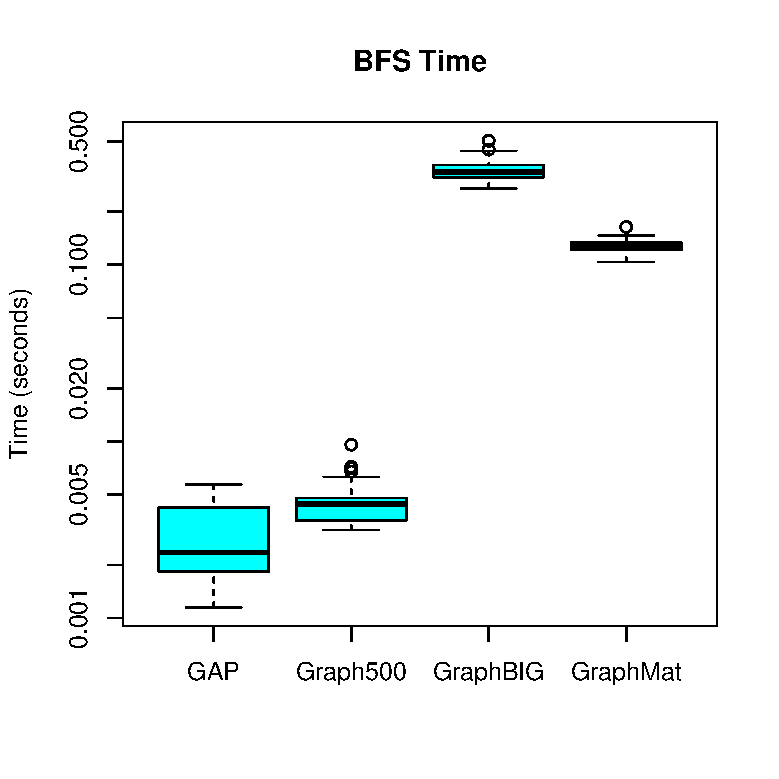
\includegraphics[width=0.8\columnwidth]{graphics/bfs_time.pdf}
	\vspace{-18pt}
	\caption{The $y$-axis is logarithmic. [TODO: Replace this with the data with non-zero degree vertices]}
	\label{fig:bfs-time}
\end{figure}

\begin{figure}
	\centering
	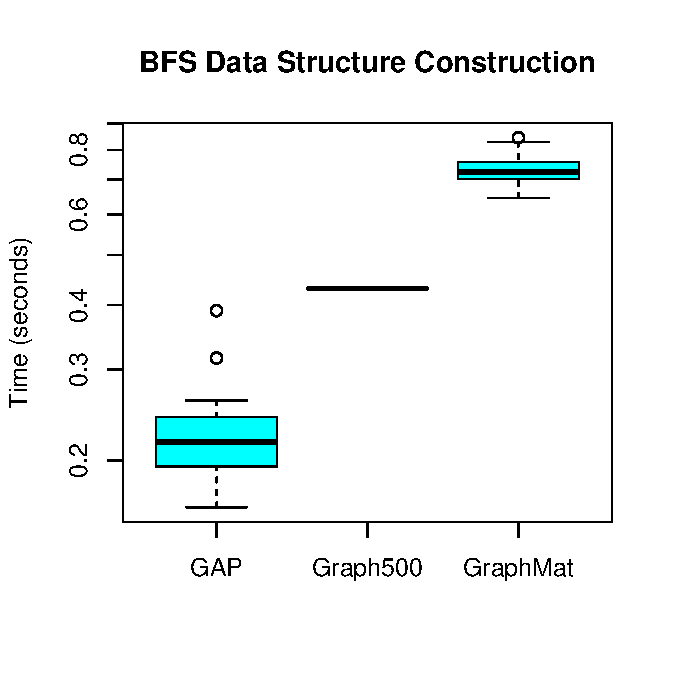
\includegraphics[width=0.8\columnwidth]{graphics/bfs_dsc.pdf}
	\vspace{-18pt}
	\caption{The $y$-axis is logarithmic. GraphBIG reads in the file and generates the data structure simultaneously so is omitted.}
	\label{fig:bfs-dsc}
\end{figure}

\begin{figure}
	\centering
	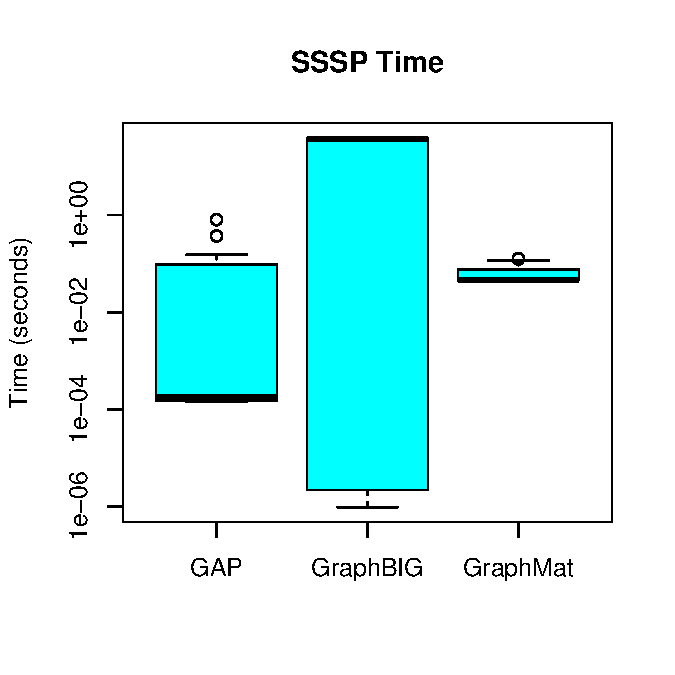
\includegraphics[width=0.8\columnwidth]{graphics/sssp_time.pdf}
	\vspace{-18pt}
	\caption{The $y$-axis is logarithmic.}
	\label{fig:sssp-time}
\end{figure}

\begin{figure}
	\centering
	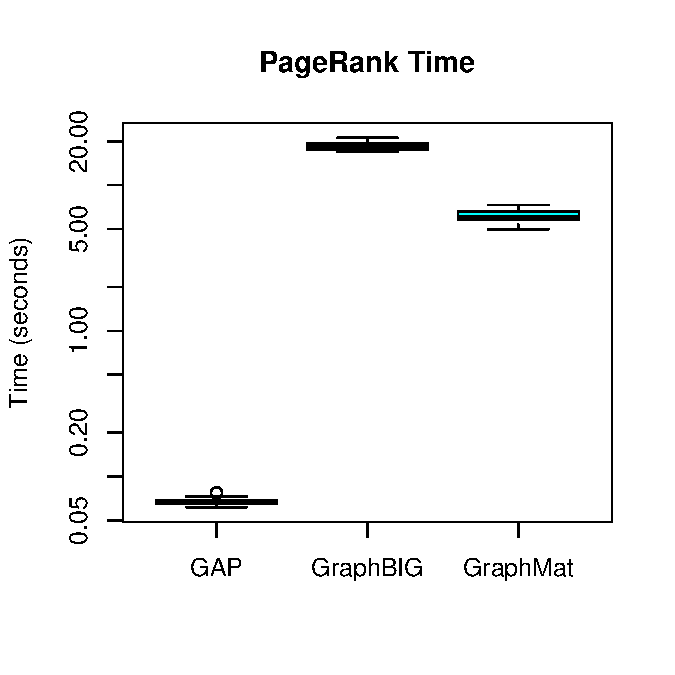
\includegraphics[width=0.8\columnwidth]{graphics/pr_time.pdf}
	\vspace{-18pt}
	\caption{The $y$-axis is logarithmic. GraphMat continues to run until none of the vertices' ranks change. [There is only one data point]}
	\label{fig:pr-time}
\end{figure}

\begin{figure}
	\centering
	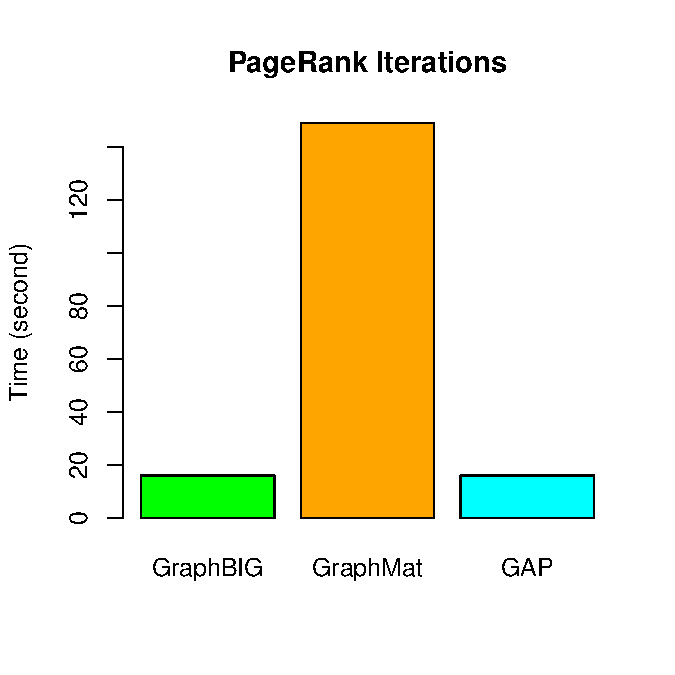
\includegraphics[width=0.8\columnwidth]{graphics/pr_iters.pdf}
	\vspace{-18pt}
	\caption{The $y$-axis \emph{not} logarithmic. GraphMat iterations are measured differently because of the ``think like a vertex'' paradigm and runs unitl none of the vertices' ranks change. [There is only one data point]}
	\label{fig:pr-iters}
\end{figure}

%\begin{table}[htb]
%	\centering
%	\begin{tabular}{l|c|c|c}
%		& BFS & SSSP & PR \\ \hline
%		Graph500 & & & \\ \hline
%		PBGL  & & & \\ \hline
%		GAP  & & & \\ \hline
%		GraphBIG  & & & \\ \hline
%		Galois  & & & \\ \hline
%		PowerGraph  & & &
%	\end{tabular}
%	\caption{Performance. Note that implementations of every algorithm are not availabe for every platform.}
%	\label{tab:reportcard}
%\end{table}

%Table~\ref{tab:perf} lists performance in milliseconds of runtime according to the graphalytics output. Graphalytics also outputs MTEPS or millions of traversed edges pers econd. However, the graphalytics version does not make sense in all cases: for example, computing the local clustering coefficient involves traversing each edge multiple times (proportional to the sparsity of the graph), while breadth first search (BFS) traverses each edge exactly once, and on na\:ive implementations single-source shortest paths (SSSP) may have $O(|E| + |V|^2)$ traversed edges.
% TODO: Cite Comer algorithm book for Dijkstra's algorithm runtime.

In Table~\ref{tab:perf}, BFS is breadth-first search, SSSP is single-source shortest paths, LCC is local clustering coefficient, PR is PageRank, CDLP is community detection using label propagation, and WCC is weakly connected components. For the algorithms used, see \cite{Iosup:2016:Graphalyticstech}.

% TODO: This should be unnecessary once autogeneration is used.
\begin{table}[!htb]
	\centering
%	\begin{tabular}{l|r|r|}
%	 & PowerGraph & OpenG \\ \hline
%	BFS & 81.8 & 341 \\ \hline
%	SSSP & 1.64 & 15.0 \\ \hline
%	LCC & 54.6 & 142 \\ \hline
%	\end{tabular}

		\centering
		\pgfplotstabletypeset[
			col sep=comma,
			string type, % Makes the .style={string type} redundant
			columns={[index]0,openg,powergraph},
			every head row/.style={after row=\midrule},
			columns/0/.style={string type, column type={l|}, column name={}},
			columns/openg/.style={string type, column type={r}},
			columns/powergraph/.style={string type, column type={r}}
		]{../report/runtime.csv}
	\caption{Performance Results for the \texttt{dota-league} dataset with 61,670 vertices and 50,870,313 edges.}
	\label{tab:perf}
\end{table}

\begin{table}[!htb]
	\centering
	\begin{tabular}{l|c|c|c}
		System & Load Graph & \begin{tabular}[x]{@{}c@{}}Construct Data \\ Structure\end{tabular} & Run BFS \\ \hline
		Graph500 & 0.3474 & 0.3971 & 0.003380 \\
		GraphBIG & 37.22  & N/A    & 0.1528 \\
		GraphMat & 0.1511 & 1.101  & 0.1031 \\
		GAP      & 2.351  & 0.1935 & 0.001393 \\
	\end{tabular}
	\caption{The above table shows times for $2^{20}$ verties and the times are in seconds. The Graph500 generates the graph instead of loading it into a file. GraphBIG builds the graph and reads in the file simultaneously. These results were averaged across 64 roots.}
	\label{tab:fileload}
\end{table}

[Compare lines of code for implementation]



\section{Graph Processing Taxonomy}
This is in the spirit of \cite{Doekemeijer:2015:GPFSurvey}. Here, ``|'' means ``or'' and ``+'' means ``and.'' FOSS means Free and Open Source Software. The quotes around ``yes'' for HPC mean that the product claims to be amenable to high performance computing. Whether these actually achieve their goal is one of the purposes of this project.
\begin{table*}[t]
	\begin{minipage}{\linewidth} % So the footnotes all get printed on the same page
		\centering
		%\small
		\pgfplotstabletypeset[
			col sep=comma,
			string type, % Makes the .style={string type} redundant
			columns={Name,Type,Parallelism,Target,FOSS,Source,Notes},
			every head row/.style={after row=\midrule},
			columns/Name/.style={string type, column type={l|}},
			columns/Type/.style={string type},
			% columns/HPC/.style={string type},
			columns/Parallelism/.style={string type},
%			columns/Comm./.style={%
%				string type,
%				postproc cell content/.style={%
%					@cell content/.add={\footnotesize}
%				}
%			},
			columns/Target/.style={string type},
			columns/FOSS/.style={string type},
			columns/Source/.style={string type},
			columns/Notes/.style={
				preproc cell content/.style={@cell content=
					\ifx&##1&% Only make a footnote if the cell is nonempty
						##1
					\else
						\footnote{##1}
					\fi}
			},
		]{../report/platforms.csv}
		\caption{Tools used for graph processing}
		\label{tab:frameworks}
	\end{minipage}
\end{table*}


\section{Conclusion} % Begin with the end in mind...
We have presented an updated survey of parallel graph processing frameworks supplementary to \cite{Doekemeijer:2015:GPFSurvey}. From this, we have selected a representative subset of frameworks on which performance is analyzed and have stored these results in a database. To facilitate parallel graph processing, hardware information and performance results are automatically populated (as were all the tables in this paper). These performance results are then used to provide simple recommendations of the optimally-performing framework given a particular algorithm and problem size.
% We have developed a simple model of hardware and its correlation with performance to predict performance on other architectures

%\bibliographystyle{acm}
\bibliographystyle{IEEEtranS}
\bibliography{../drp}
\end{document}
